%==============================================================
%  System Identification of a Nonlinear Dynamical System
%  Course: Machine Learning for Vision and Multimedia, PoliTO 25/26
%  Project 2.5 -- Cortical Responses Evoked by Wrist Joint Manipulation
%  CVPR 2020 author-kit format
%==============================================================
\documentclass[10pt,twocolumn,letterpaper]{article}

\usepackage{cvpr}
\usepackage{times}
\usepackage{epsfig}
\usepackage{graphicx}
\usepackage{amsmath}
\usepackage{amssymb}
\usepackage{booktabs}

% Include other packages here, before hyperref.

\usepackage[pagebackref=true,breaklinks=true,letterpaper=true,colorlinks,bookmarks=false]{hyperref}

\cvprfinalcopy % *** Uncomment this line for the final submission

\def\cvprPaperID{****} % *** Enter the CVPR Paper ID here
\def\httilde{\mbox{\tt\raisebox{-.5ex}{\symbol{126}}}}

% Pages are numbered in submission mode, and unnumbered in camera-ready
\ifcvprfinal\pagestyle{empty}\fi

\begin{document}

%%%%%%%%% TITLE
\title{Neural-Network System Identification of Cortical Responses to
       Wrist Joint Perturbations: A Comparison of NNARX, RNN, LSTM and
       GRU Models}

\author{Fabio Brugiafreddo\\
Politecnico di Torino\\
Machine Learning for Vision and Multimedia, A.Y. 2025/26\\
{\tt\small brugia.fabio@gmail.com}
}

\maketitle
%\thispagestyle{empty}

%%%%%%%%% ABSTRACT
\begin{abstract}
   We address the data-driven identification of the nonlinear
   single-input single-output (SISO) mapping between a wrist-joint
   angular perturbation and the top-SNR independent component of the
   evoked electroencephalographic (EEG) response, using the publicly
   available Vlaar \etal benchmark. We compare four families of neural
   models---a Nonlinear Auto-Regressive network with eXogenous inputs
   (NNARX), a vanilla Recurrent Neural Network (RNN), a Long Short-Term
   Memory network (LSTM) and a Gated Recurrent Unit network (GRU)---on
   three tasks of increasing difficulty: one-step ahead prediction,
   $k$-step ahead prediction, and full free-run simulation. All models
   share a common preprocessing pipeline that reproduces the original
   MATLAB reference, and a unified training, evaluation and budgeting
   protocol. We report accuracy (NRMSE and VAF), parameter count, FLOPs
   per output sample and wall-clock training time. On one-step
   prediction all models reach $\mathrm{VAF}\geq 75\%$, but in
   closed-loop simulation only the NNARX family is competitive, with the
   NNARX-FROLS variant peaking at $\mathrm{VAF}\approx 27\%$, while
   RNN/LSTM/GRU collapse below $7\%$. The gap relative to the published
   Volterra and NARMAX baselines ($\mathrm{VAF}\approx 46\%$) is
   discussed and traced back to the mismatch between teacher-forced
   training and free-run evaluation, the limited size of the dataset and
   the absence of scheduled sampling for the recurrent models. As a
   complementary experiment, we evaluate the same checkpoints in
   \emph{Kalman-assisted} free-run mode, in which a small fraction
   ($\alpha=0.15$) of the true output is mixed back into the
   autoregressive feedback at each step. Under this regime the
   NNARX-FROLS variant climbs to $\mathrm{VAF}\approx 58\%$, exceeding
   the published Volterra baseline, and the previously collapsing RNN
   recovers to $\mathrm{VAF}\approx 35\%$.
\end{abstract}

%%%%%%%%% BODY TEXT
%==============================================================
\section{Introduction}

\subsection{Context and motivation}
System identification---the data-driven construction of a mathematical
model of a dynamical system from measured input/output data---is a
foundational problem at the intersection of control theory, signal
processing and machine learning~\cite{Ljung1999,Nelles2001,Sjoberg1995}.
When the underlying dynamics are linear, the theory is mature and a
handful of canonical model structures (ARX, ARMAX, state-space) cover
most practical cases. The picture is far less settled for
\emph{nonlinear} systems, where no single parameterisation is
universally adequate and the modeller must trade off expressiveness,
identifiability, data efficiency and computational cost. The classical
nonlinear pipeline first commits to a regressor structure---a polynomial
NARMAX expansion, a Volterra series, a wavelet or radial-basis
dictionary---and then estimates its coefficients. Deep learning has
recently emerged as an attractive alternative that folds both the
structural choice and the parameter estimation into a single end-to-end
trainable model~\cite{Andersson2019,Forgione2021}, at the price of
weaker interpretability and a less transparent inductive bias.

\subsection{Why a biomedical benchmark}
Biomedical signals constitute a particularly demanding test bed for
nonlinear identification: the signal-to-noise ratio is low, the
inter-subject variability is large, and the generating physiology is, at
best, only partially understood. The benchmark introduced by
Vlaar \etal~\cite{Vlaar2018}---the cortical response, measured by
electroencephalography (EEG), evoked by a mechanical perturbation of the
wrist joint---is an attractive case study for three reasons. First,
after independent-component analysis the input/output pair reduces to a
clean single-input single-output (SISO) mapping between the handle angle
$u[k]$ and the highest-SNR cortical component $y[k]$. Second, the
acquisition protocol is fully documented, publicly released, and
reproducible. Third, several model classes have already been evaluated
on it, providing strong external baselines against which a new method
can be calibrated~\cite{Vlaar2018,Gu2018,Gu2021,Santos2023}. Beyond its
role as a benchmark, accurate forward models of stimulus-evoked cortical
activity are of practical interest for closed-loop neurorehabilitation
and brain--computer interfaces, where a predictive model of the neural
response can inform stimulation timing and decoding.

\subsection{Limitations of existing approaches}
The published literature on this benchmark is dominated by
\emph{polynomial} system-identification methods. The original
study~\cite{Vlaar2018} fits subject-specific second-order Volterra
series; Gu \etal~\cite{Gu2021} couple a polynomial NARMAX structure with
FROLS term selection, and~\cite{Gu2018} adds a small hierarchical neural
network on top of the NARMAX regressors. These works share three
features that, taken together, leave a gap. (i)~They report results
almost exclusively in \emph{one-step-ahead} (or low-order $k$-step)
prediction, where past \emph{true} outputs are always available to the
model; the much harder \emph{free-run} (closed-loop) simulation regime,
in which the model is fed back its own predictions, is rarely
characterised. (ii)~The models are fitted \emph{subject-specifically},
which inflates the reported accuracy and sidesteps the question of how a
model generalises to an unseen subject. (iii)~Despite the popularity of
recurrent neural networks (RNN, LSTM, GRU) elsewhere in sequence
modelling, no systematic head-to-head comparison of the standard neural
families used in identification (NNARX, vanilla RNN, LSTM, GRU) has been
carried out on this benchmark under a single, shared preprocessing and
evaluation protocol. In particular, the well-known mismatch between
teacher-forced training and free-run inference~\cite{Bengio2015}---and
the failure modes it induces in recurrent simulators---has not been
quantified on this data.

\subsection{Proposed approach and added value}
This paper addresses that gap. We perform a controlled, reproducible
comparison of the four standard neural model families for nonlinear
identification---NNARX, RNN, LSTM and GRU---on the Vlaar~2018 benchmark,
under a single configuration-driven pipeline that faithfully reproduces
the original MATLAB preprocessing. Crucially, every model is evaluated
not only in the easy one-step regime but also in three-step prediction
and in full \emph{free-run simulation}, and is additionally budgeted in
terms of parameter count, analytical FLOPs per output sample and
wall-clock training time, so that accuracy is always reported jointly
with cost. To probe generalisation rather than memorisation, we adopt a
Leave-One-Subject-Out (LOSO) protocol as the main reporting setting. Our
analysis reveals a sharp and, at first sight, counter-intuitive
phenomenon: while all families reach $\mathrm{VAF}\geq 75\%$ in one-step
prediction, only the NNARX family remains usable once the loop is
closed, whereas the recurrent models collapse towards a trivial
attractor. We trace this back to the training/inference mismatch and, as
a complementary diagnostic, show that re-injecting as little as $15\%$
of the true output into the autoregressive feedback (a steady-state,
$\alpha$-$\beta$ Kalman form) recovers most of the lost accuracy---a
strong indication that the dominant error source is closed-loop drift
rather than insufficient model capacity.

\subsection{Contributions}
The contributions of this work are the following:
\begin{itemize}
    \item A reproducible re-implementation of the Vlaar~2018
          preprocessing pipeline, organised as a single,
          configuration-driven Jupyter notebook that runs unmodified
          locally and on Kaggle.
    \item A unified training and evaluation protocol that, for each of
          the four neural families, reports accuracy in three regimes
          (one-step, three-step and full free-run simulation) together
          with parameter count, analytical FLOPs per output sample and
          wall-clock training time, under both within-subject and
          Leave-One-Subject-Out splits.
    \item An architectural sweep (hidden size, depth, regressor width
          and FROLS term count) that shows the free-run accuracy of each
          family to be limited by the training objective rather than by
          model capacity.
    \item A quantitative analysis of the teacher-forcing/free-run gap,
          including a Kalman-assisted simulation experiment that
          isolates closed-loop drift from model misspecification and, at
          $\alpha=0.15$, lifts the best NNARX variant above the
          published Volterra baseline.
\end{itemize}

\subsection{Outline}
The remainder of the paper is organised as follows.
Section~\ref{sec:method} presents the methodology and system
architecture: the problem formalism, the data and preprocessing pipeline,
the four predictive model families, the training and inference
strategies, and the evaluation metrics. Section~\ref{sec:exp} reports the
experimental results across the three phases and the Kalman-assisted
experiment. Section~\ref{sec:rw} then positions these results against the
polynomial and neural system-identification literature on the same
benchmark. Section~\ref{sec:discussion} discusses the findings and the
gap with the literature, and Section~\ref{sec:conclusion} concludes.

%==============================================================
\section{Methodology and System Architecture}\label{sec:method}

\subsection{System overview}\label{sec:overview}
The identification system is organised as a single, linear pipeline whose
stages are driven by one global configuration dictionary, so that every
experiment in Section~\ref{sec:exp} is obtained by overriding a small set
of fields rather than by editing code. The four stages are: \textbf{(S1)}
a preprocessing front-end that maps the raw multi-period EEG recordings
into a normalised SISO input/output tensor (Section~\ref{sec:data});
\textbf{(S2)} a representation stage that builds, from that tensor, either
an explicit lagged regressor (for the NNARX family) or a raw input
sequence (for the recurrent family); \textbf{(S3)} a parametric model
$f_\theta$ drawn from one of four families (NNARX, RNN, LSTM, GRU,
Section~\ref{sec:models}); and \textbf{(S4)} an inference-and-budgeting
stage that runs the trained model in three regimes---one-step, $k$-step
and free-run simulation---and records accuracy together with parameter
count, analytical FLOPs and wall-clock time
(Sections~\ref{sec:infer}--\ref{sec:metrics}). The block structure is
sketched in Fig.~\ref{fig:arch}.

\begin{figure}[t]
\centering
% \includegraphics[width=0.95\linewidth]{figures/architecture.pdf}
\fbox{\rule{0pt}{3.2cm}\rule{0.85\linewidth}{0pt}}
\caption{System architecture. Raw EEG recordings (S1) are preprocessed
into a normalised SISO tensor, from which either a lagged regressor or a
raw sequence is built (S2); a parametric model $f_\theta$ (S3) is trained
by a $k$-step curriculum and evaluated in three inference regimes with a
cost budget (S4).}
\label{fig:arch}
\end{figure}

\subsection{Problem formulation}\label{sec:formulation}
We model a single-input single-output (SISO), discrete-time, causal,
time-invariant nonlinear dynamical system. Let $u[k]\in\mathbb{R}$ denote
the (preprocessed) wrist-handle angle and $y[k]\in\mathbb{R}$ the
top-SNR cortical component at sample index $k$, with sampling period
$T_s=1/f_s$ and $f_s=256~\mathrm{Hz}$. We assume the data-generating
process admits a finite-memory nonlinear auto-regressive representation
with exogenous input,
\begin{equation}
    y[k] = g\big(\varphi[k]\big) + e[k],
    \label{eq:plant}
\end{equation}
where $e[k]$ collects measurement noise and unmodelled dynamics, $g$ is
an unknown nonlinear map, and $\varphi[k]$ is the \emph{regressor vector}
\begin{equation}
    \varphi[k] =
    \big[\,
      \underbrace{u[k],\dots,u[k-n_u+1]}_{n_u\text{ input taps}},\;
      \underbrace{y[k-1],\dots,y[k-n_y]}_{n_y\text{ output taps}}
    \,\big]^{\!\top}
    \in \mathbb{R}^{\,n_u+n_y}.
    \label{eq:regressor}
\end{equation}
The identification problem is to find parameters $\theta$ of a model
$f_\theta$ that approximate $g$. We sharply distinguish two operating
modes, which differ only in how the output taps of $\varphi[k]$ are
populated:
\begin{itemize}
    \item the \textbf{one-step-ahead predictor}
          $\hat{y}[k\,|\,k-1]=f_\theta(\varphi[k])$, in which the output
          taps are the \emph{measured} past outputs $y[k-j]$;
    \item the \textbf{simulation (free-run) model}
          $\hat{y}_s[k]=f_\theta(\hat\varphi[k])$, in which the output
          taps are the model's \emph{own} past predictions
          $\hat{y}_s[k-j]$ (Section~\ref{sec:infer}).
\end{itemize}
Equivalently, the recurrent models adopt the \emph{state-space} form
\begin{equation}
    h[k] = \psi\big(h[k-1],u[k]\big), \qquad
    \hat{y}[k] = W_o\,h[k] + b_o,
    \label{eq:statespace}
\end{equation}
with internal state $h[k]\in\mathbb{R}^{H}$; here the autoregressive
memory of \eqref{eq:regressor} is replaced by the latent state $h[k]$,
and \eqref{eq:statespace} is closed-loop by construction.

\subsection{Data and preprocessing}\label{sec:data}
We use the medium-size version of the public benchmark \emph{Cortical
Responses Evoked by Wrist Joint
Manipulation}~\cite{Vlaar2018,VlaarDataset}: \emph{$S=10$ subjects}, each
performing \emph{$M=7$ realisations} of $30~\mathrm{s}$, recorded at
$f_{s,\mathrm{raw}}=2048~\mathrm{Hz}$. The input is the angular handle
perturbation; the output is, after independent-component analysis, the
cortical component with the highest signal-to-noise ratio across
realisations. Our preprocessing is a Python port of the reference MATLAB
script \texttt{Load\_Plot\_EEG\_2.m} and, applied independently per
subject $s$, performs: (1)~averaging over the $P$ periods of each
realisation to suppress stimulus-locked noise; (2)~downsampling by a
factor $8$ to $f_s=256~\mathrm{Hz}$; (3)~per-subject mean removal; (4)
amplitude normalisation by
\begin{equation}
    \sigma_s = \frac{1}{M}\sum_{m=1}^{M}
               \operatorname{std}_k\big(y_{s,m}[k]\big),
    \label{eq:norm}
\end{equation}
the mean across realisations of the per-realisation standard deviation;
and (5)~a circular shift of $5$ samples ($\approx 19.5~\mathrm{ms}$)
applied to the input to compensate for the known stimulus-to-cortex
latency. The result is a tensor of shape $[S,M,N]=[10,7,N]$ with the time
axis last.

For evaluation we use two protocols. In the \textbf{within-subject}
split, each subject contributes $6$ realisations to training and $1$ to
test, as in~\cite{Gu2021}. In the \textbf{Leave-One-Subject-Out (LOSO)}
split, one full subject is held out and the remaining $9$ form the
training set; this exposes inter-subject variability and is our main
reporting setting. After splitting, each branch is flattened to
$[\text{num\_sequences},N]$, so all downstream code is split-agnostic.

\subsection{Predictive models}\label{sec:models}
All four families produce the scalar prediction $\hat{y}[k]$; they differ
in how they parameterise $f_\theta$.

\subsubsection{NNARX}
The NNARX model instantiates \eqref{eq:plant} with $f_\theta$ a
multilayer perceptron (MLP) over the regressor \eqref{eq:regressor},
\begin{equation}
    \hat{y}[k] = W_3\,\rho\big(W_2\,\rho(W_1\varphi[k]+b_1)+b_2\big)+b_3,
    \label{eq:nnarx}
\end{equation}
with two hidden layers of width $(64,64)$, GELU activation $\rho$ and
dropout $0.1$. We adopt the dense tap structure $(n_u,n_y)=(20,5)$
of~\cite{Gu2021}, so $\varphi[k]\in\mathbb{R}^{25}$. To reduce
overfitting we average an ensemble of $E=3$ independently initialised
networks at test time, $\hat{y}=\tfrac{1}{E}\sum_{e}\hat{y}^{(e)}$.

\paragraph{FROLS regressor selection.}
The \textbf{NNARX-FROLS} variant prunes the regressor before the MLP. Let
$\mathcal{D}=\{\varphi_j\}_{j=1}^{n_u+n_y}$ be the candidate taps. Forward
Regression with Orthogonal Least Squares~\cite{Gu2021} orthogonalises the
candidates and, at each step, selects the term maximising the Error
Reduction Ratio
\begin{equation}
    \mathrm{ERR}_j =
    \frac{\big(\langle q_j, y\rangle\big)^2}
         {\langle q_j,q_j\rangle\,\langle y,y\rangle},
    \label{eq:err}
\end{equation}
where $q_j$ is the component of $\varphi_j$ orthogonal to the
already-selected terms. The procedure stops after $k\in\{10,20,40\}$
terms; only the retained taps feed \eqref{eq:nnarx}.

\subsubsection{Recurrent state-space models}
The recurrent family realises \eqref{eq:statespace} with a single layer
of hidden size $H=64$ and a linear read-out $W_o\in\mathbb{R}^{1\times
H}$. The three cell types differ only in the state-update map $\psi$. The
\textbf{Elman RNN}~\cite{Elman1990} uses
\begin{equation}
    h[k] = \tanh\!\big(W_{ih}\,u[k] + W_{hh}\,h[k-1] + b_h\big).
    \label{eq:rnn}
\end{equation}
The \textbf{LSTM}~\cite{Hochreiter1997} augments the state with a memory
cell $c[k]$ and three gates,
\begin{align}
    i[k] &= \sigma\!\big(W_i\,u[k]+U_i\,h[k-1]+b_i\big), \notag\\
    f[k] &= \sigma\!\big(W_f\,u[k]+U_f\,h[k-1]+b_f\big), \notag\\
    o[k] &= \sigma\!\big(W_o^{g}\,u[k]+U_o\,h[k-1]+b_o^{g}\big),
    \label{eq:lstm}\\
    \tilde{c}[k] &= \tanh\!\big(W_c\,u[k]+U_c\,h[k-1]+b_c\big), \notag\\
    c[k] &= f[k]\odot c[k-1] + i[k]\odot\tilde{c}[k], \quad
    h[k] = o[k]\odot\tanh c[k], \notag
\end{align}
where $\sigma$ is the logistic sigmoid and $\odot$ the Hadamard product.
The \textbf{GRU}~\cite{Cho2014} merges memory and output into a single
state through reset/update gates,
\begin{align}
    r[k] &= \sigma\!\big(W_r u[k]+U_r h[k-1]+b_r\big), \notag\\
    z[k] &= \sigma\!\big(W_z u[k]+U_z h[k-1]+b_z\big), \label{eq:gru}\\
    \tilde{h}[k] &= \tanh\!\big(W_h u[k]+U_h(r[k]\odot h[k-1])+b_h\big),
    \notag\\
    h[k] &= (1-z[k])\odot h[k-1] + z[k]\odot\tilde{h}[k]. \notag
\end{align}
Because the latent state carries the autoregressive information, a
forward pass over a test sequence \emph{is} already the free-run
simulation: no teacher forcing is applied to recurrent models at
evaluation time.

\subsection{Training strategy}\label{sec:training}
All models are trained by minimising a \emph{multi-step} (curriculum)
loss that directly targets simulation rather than one-step accuracy.
Given a training sequence, a random start index $t$ and a horizon $K$,
we generate a length-$K$ roll-out $\hat{y}[t{+}i]$, $i=0,\dots,K-1$, by
feeding back predictions---through $\hat\varphi$ for NNARX
\eqref{eq:nnarx} or through the recurrent state \eqref{eq:statespace}---
and minimise
\begin{equation}
    \mathcal{L}_K
    = \mathbb{E}_{t}\!\left[\frac{1}{K}\sum_{i=0}^{K-1}
      \big(\hat{y}[t{+}i]-y[t{+}i]\big)^2\right].
    \label{eq:loss}
\end{equation}
The horizon follows a curriculum that is progressively lengthened,
$K\in\{1,5,10,20,40,80,160,320\}$ for NNARX and up to $K=1024$ for the
recurrent models; $K=1$ recovers ordinary teacher-forced one-step
training. Optimisation uses Adam, gradient clipping at norm $1.0$, cosine
learning-rate decay, and a warm-up window of $\max(n_u,n_y)$ samples
(NNARX) or $10$ samples (recurrent) during which the loss is not
accumulated.

\subsection{Inference: free-run and innovation feedback}\label{sec:infer}
\paragraph{Pure free-run simulation.}
At test time the model is run in closed loop. The first
$w=\max(n_u,n_y)$ (NNARX) or $w=10$ (recurrent) output samples are taken
from the ground truth as warm-up; thereafter the model is iterated with
its own predictions,
\begin{equation}
    \hat{y}_s[k] = f_\theta(\hat\varphi[k]), \qquad
    \hat\varphi[k]\ \text{built from}\ \{u[\cdot],\hat{y}_s[k-j]\},
    \label{eq:freerun}
\end{equation}
for $k>w$. This is the most demanding regime and the one most relevant to
deployment when no online measurement of $y$ is available.

\paragraph{Innovation feedback (mitigation strategy).}
To quantify how much of the free-run error is due to autoregressive drift
rather than to model misspecification, we introduce a soft closed-loop
correction. At each step a fraction of the true output is mixed back into
the fed-back value through the \emph{innovation}
$\nu[k]=y[k]-\hat{y}[k]$,
\begin{equation}
    \tilde{y}[k] = \hat{y}[k] + \alpha\,\big(y[k]-\hat{y}[k]\big),
    \qquad \alpha\in[0,1],
    \label{eq:kalman}
\end{equation}
and $\tilde{y}[k-j]$ replaces $\hat{y}_s[k-j]$ in \eqref{eq:freerun}.
Equation~\eqref{eq:kalman} is the steady-state form of a scalar Kalman
filter: for a random-walk output model with process variance $Q$ and
measurement variance $R$, the Kalman update $\hat{x}=\hat{x}^-+
K(y-\hat{x}^-)$ has a constant gain $K=\alpha$ once the error covariance
reaches steady state, which is also the $\alpha$-$\beta$
filter~\cite{Brookner1998}. The limits $\alpha\!=\!0$ and $\alpha\!=\!1$
recover pure free-run and full one-step teacher forcing, respectively;
intermediate $\alpha$ anchors the simulation with only a fraction of the
sensor information. We use a fixed $\alpha=0.15$ and reuse the
Section~\ref{sec:training} checkpoints \emph{without} retraining.

\subsection{Evaluation metrics and cost budgeting}\label{sec:metrics}
\paragraph{Accuracy.}
Let $y,\hat{y}\in\mathbb{R}^N$ be reference and prediction on a held-out
realisation. We report the Normalised Root-Mean-Squared Error and the
Variance Accounted For,
\begin{equation}
    \mathrm{NRMSE} = \frac{\|y-\hat{y}\|_2}{\|y-\bar y\|_2}, \quad
    \mathrm{VAF} = \max\!\Big(0,\,1-\tfrac{\mathrm{var}(y-\hat{y})}
    {\mathrm{var}(y)}\Big)\!\cdot\!100\%,
    \label{eq:metrics}
\end{equation}
the latter being the standard metric of~\cite{Vlaar2018,Gu2018,Gu2021}.
Each is computed in three regimes: \textbf{(i)} one-step ahead (OSA),
true past outputs supplied; \textbf{(ii)} three-step ahead ($\approx
12~\mathrm{ms}$); and \textbf{(iii)} free-run simulation
\eqref{eq:freerun}.

\paragraph{Complexity.}
We report the trainable-parameter count and the analytical number of
floating-point operations per output sample. Counting one multiply-add as
$2$ FLOPs, an MLP with layer widths $d_0,\dots,d_L$ costs
$F_{\text{MLP}}=2\sum_{\ell=1}^{L} d_{\ell-1}d_\ell$ plus the
element-wise activations; a recurrent cell with input dimension $d$ and
hidden size $H$ costs
\begin{equation}
    F_{\text{cell}} = 2\,G\,H\,(d+H) + c_{\mathrm{nl}}H + 2H,
    \label{eq:flops}
\end{equation}
where $G\!\in\!\{1,3,4\}$ for RNN/GRU/LSTM is the number of gates,
$c_{\mathrm{nl}}H$ accounts for the gate non-linearities and the final
$2H$ for the linear read-out. We use the closed form \eqref{eq:flops}
because off-the-shelf tools such as \texttt{ptflops} miss the gate-wise
structure of the LSTM and GRU updates. Finally we report wall-clock
training time on identical hardware (a consumer GPU is auto-detected,
otherwise CPU).

%==============================================================
\section{Experimental Setup and Results}\label{sec:exp}

\subsection{Experimental setup}\label{sec:setup}
\paragraph{Environment.}
All experiments are produced by a single configuration-driven Jupyter
notebook (\texttt{project-si-mlicv.ipynb}) built on PyTorch, with the
compute device auto-detected (a consumer GPU when available, otherwise
CPU). Every reported number is read back from a JSON snapshot
(\texttt{phase1\_metrics.json} for Phase~1, \texttt{phase2\_rec.json} for
the recurrent sweep, \texttt{loso\_folds.json} for the cross-validation),
so the tables below are reproducible by re-executing the notebook. The
NNARX family is reported as an ensemble of $E=3$ networks; the Phase~2
recurrent sweep is averaged over $3$ random seeds and we report the
standard deviation across seeds.

\paragraph{Compared methods.}
We benchmark the four neural families of Section~\ref{sec:models}
(NNARX, NNARX-FROLS, RNN, LSTM, GRU) against two \emph{classical}
system-identification baselines that share the same regressor
$(n_u,n_y)=(20,5)$: a linear least-squares \textbf{ARX} model and a
degree-$2$ \textbf{polynomial NARMAX}. The classical baselines act as the
``standard approach'' reference against which the added value of the
neural models is measured.

\paragraph{Test scenarios.}
Each method is evaluated in the three inference regimes of
Section~\ref{sec:metrics}---one-step ahead (OSA), three-step ahead, and
full free-run simulation---under both the within-subject and the LOSO
protocol of Section~\ref{sec:data}. The main accuracy/cost comparison
(Phase~1, Table~\ref{tab:phase1}) and the architectural sweep (Phase~2,
Table~\ref{tab:phase2}) are reported on the held-out test set; the
cross-validated LOSO numbers are summarised in Section~\ref{sec:phase3}.
The key hyper-parameters held fixed across all runs are listed in
Table~\ref{tab:hparams}.

\begin{table}[t]
\centering
\caption{Fixed hyper-parameters shared across all experiments.}
\label{tab:hparams}
\setlength{\tabcolsep}{4pt}
\begin{tabular}{ll}
\toprule
\textbf{Component} & \textbf{Setting} \\
\midrule
Sampling rate $f_s$ & $256~\mathrm{Hz}$ \\
Regressor taps $(n_u,n_y)$ & $(20,5)$ \\
NNARX MLP & widths $(64,64)$, GELU, dropout $0.1$ \\
NNARX ensemble $E$ & $3$ \\
FROLS retained terms $k$ & $\{10,20,40\}$ \\
Recurrent hidden size $H$ & $64$ (swept $\{16,32,64,128\}$) \\
Recurrent layers & $1$ (swept $\{1,2\}$) \\
Optimiser & Adam, gradient clip $1.0$ \\
LR schedule & cosine decay \\
Curriculum horizon $K$ & up to $320$ (NNARX) / $1024$ (rec.) \\
Innovation gain $\alpha$ & $0.15$ \\
\bottomrule
\end{tabular}
\end{table}

\subsection{Phase 1: head-to-head baseline}\label{sec:phase1}

Table~\ref{tab:phase1} reports the Phase~1 results on the held-out test
set, comparing the two classical baselines (top block) with the four
neural families (bottom block). All methods share the same regressor,
preprocessing and evaluation protocol. The numbers are produced by the
companion notebook \texttt{project-si-mlicv.ipynb} and correspond exactly
to the JSON snapshot \texttt{phase1\_metrics.json}.

\begin{table*}[t]
\centering
\caption{Phase 1 -- head-to-head comparison on the held-out test set.
Top block: classical baselines; bottom block: neural families. Lower
NRMSE is better, higher VAF is better. ``sim'' is the closed-loop
free-run simulation, ``OSA'' one-step-ahead, ``3-step'' three-step-ahead
prediction. ``div.'' marks a free-run that diverges. Best value per
column in bold.}
\label{tab:phase1}
\begin{tabular}{lcccccccc}
\toprule
\textbf{Model} & \textbf{Params} & \textbf{FLOPs/sample} &
\textbf{Train [s]} &
\textbf{NRMSE\textsubscript{sim}} & \textbf{VAF\textsubscript{sim}} &
\textbf{NRMSE\textsubscript{OSA}} & \textbf{VAF\textsubscript{OSA}} &
\textbf{VAF\textsubscript{3-step}} \\
\midrule
ARX (linear)         &     25 &     50 &  0.00 & 0.988 &  2.4\%   & 0.450 & 79.7\% & --     \\
PolyNARMAX (deg.\ 2) &     15 &     30 &  2.58 & 3.142 & div.     & 0.506 & 74.4\% & 22.5\% \\
\midrule
NNARX           &  5\,889 & 34\,947 & 55.36 & 0.945 & 10.9\% & 0.451 & 79.7\% & 22.5\% \\
NNARX-FROLS ($k=10$) & 5\,185 & 30\,723 & 11.59 & 0.861 & 25.9\% & 0.436 & 81.0\% & 16.8\% \\
NNARX-FROLS ($k=20$) & 5\,569 & 33\,027 &  6.80 & 0.863 & 25.5\% & \textbf{0.392} & \textbf{84.7\%} & \textbf{28.6\%} \\
NNARX-FROLS ($k=40$) & 6\,849 & 40\,707 & 11.42 & \textbf{0.853} & \textbf{27.2\%} & 0.400 & 84.0\% & 27.0\% \\
RNN             &  4\,417 &  8\,641 & 10.01 & 0.986 &  2.7\% & 0.493 & 75.7\% & 18.8\% \\
LSTM            & 17\,473 & 34\,497 & 17.49 & 0.967 &  6.5\% & 0.491 & 75.9\% & 21.9\% \\
GRU             & 13\,121 & 25\,857 & 18.03 & 0.974 &  5.2\% & 0.485 & 76.5\% & 24.1\% \\
\bottomrule
\end{tabular}
\end{table*}

Four observations are worth highlighting.

\noindent\textbf{Neural models add value over the classical baselines.}
The linear ARX already explains the one-step response well
($\mathrm{VAF_{OSA}}=79.7\%$) but is almost useless in free run
($\mathrm{VAF_{sim}}=2.4\%$), and the degree-$2$ polynomial NARMAX is
unstable in closed loop (its free-run diverges, $\mathrm{NRMSE_{sim}}=
3.14$). The best neural model, NNARX-FROLS, improves the free-run VAF by
more than an order of magnitude over ARX ($27.2\%$ vs $2.4\%$) while
keeping a comparable one-step accuracy, which is precisely the regime
that matters for simulation.

\noindent\textbf{One-step prediction is easy.} All models reach
$\mathrm{VAF_{OSA}}\geq 75\%$. Within a single ICA component the cortical
response is, after subtraction of the per-subject mean and proper
amplitude normalisation, well explained even by a short nonlinear
regressor. The differences between models are confined to a few
percentage points and well within the expected inter-subject variance.

\noindent\textbf{Free-run simulation separates the families.} The
picture changes radically as soon as we close the loop. The NNARX family
remains usable---its best variant, NNARX-FROLS with $k=40$ retained
regressors, reaches $\mathrm{VAF_{sim}}=27.2\%$---while the recurrent
models collapse below $7\%$. This is a textbook manifestation of the
\emph{training/inference mismatch}: teacher-forced training rewards
short-horizon accuracy and does not penalise the accumulation of errors
that becomes visible only in closed loop.

\noindent\textbf{Cost picture.} Among the four neural families, the RNN
is by far the cheapest ($8.6$\,kFLOPs/sample) but also the weakest in
free-run; the NNARX-FROLS ($k=20$) variant offers the best accuracy-cost
trade-off, with $33$~kFLOPs/sample, the best one-step VAF and the best
three-step VAF of the whole table.

\subsection{Phase 2: architectural sweep}\label{sec:phase2}

In Phase~2 we sweep the most relevant architectural parameter of each
family, holding the rest of the configuration fixed.

\noindent\textbf{NNARX.} We vary the MLP width between $(32,32)$,
$(64,64)$ and $(128,128)$, and the number of FROLS-retained regressors
$k\in\{10,20,40\}$. The dominant trend is that the free-run VAF plateaus
around $25$--$27\%$: increasing the width beyond $(64,64)$ does not bring
further gains, while reducing $k$ below $20$ slightly hurts the
three-step VAF. The pattern is consistent with a regime in which the
bottleneck is the loss function, not the function approximator.

\noindent\textbf{Recurrent.} We sweep the hidden size $\{32,64,128\}$ and
the number of stacked layers $\{1,2\}$, averaging over $3$ seeds
(Table~\ref{tab:phase2}). None of the $18$ configurations brings the
free-run VAF above $\approx 6\%$ (the best is GRU, $H{=}64$, single layer,
$\mathrm{VAF_{sim}}=5.9\%$). Increasing capacity does not help and often
hurts: the two-layer, $H{=}128$ cells---two orders of magnitude larger in
parameter count---collapse back to $\mathrm{VAF_{sim}}\approx 2\%$ and
their one-step VAF actually \emph{drops} (e.g.\ LSTM $H{=}64$, $L{=}2$
falls to $\mathrm{VAF_{OSA}}=62\%$), a clear sign of over-fitting rather
than under-capacity. The free-run failure of the recurrent family is
therefore not a capacity problem.

\begin{table}[t]
\centering
\caption{Phase 2 -- recurrent architectural sweep (single-layer
configurations; mean over $3$ seeds, std in parentheses). The best
free-run VAF of the whole sweep is in bold. Two-layer variants (omitted
for space) are never better and are discussed in the text.}
\label{tab:phase2}
\setlength{\tabcolsep}{4pt}
\begin{tabular}{llccc}
\toprule
\textbf{Cell} & \textbf{$H$} & \textbf{Params} &
\textbf{VAF\textsubscript{sim}} & \textbf{VAF\textsubscript{OSA}} \\
\midrule
RNN  &  32 &  1\,185 & 2.2 (0.1) & 76.6 (0.4) \\
RNN  &  64 &  4\,417 & 2.5 (0.1) & 76.2 (0.1) \\
RNN  & 128 & 17\,025 & 2.5 (0.1) & 76.1 (0.2) \\
LSTM &  32 &  4\,641 & 4.2 (1.4) & 72.1 (1.4) \\
LSTM &  64 & 17\,473 & 4.3 (0.9) & 75.2 (0.3) \\
LSTM & 128 & 67\,713 & 3.4 (1.5) & 75.4 (0.7) \\
GRU  &  32 &  3\,489 & 4.7 (1.4) & 72.9 (1.8) \\
GRU  &  64 & 13\,121 & \textbf{5.9 (1.0)} & 75.0 (0.4) \\
GRU  & 128 & 50\,817 & 4.3 (2.9) & 74.2 (1.5) \\
\bottomrule
\end{tabular}
\end{table}

A schematic visualisation of the sweep is given in
Fig.~\ref{fig:phase2} (placeholder).

\begin{figure}[t]
\centering
% 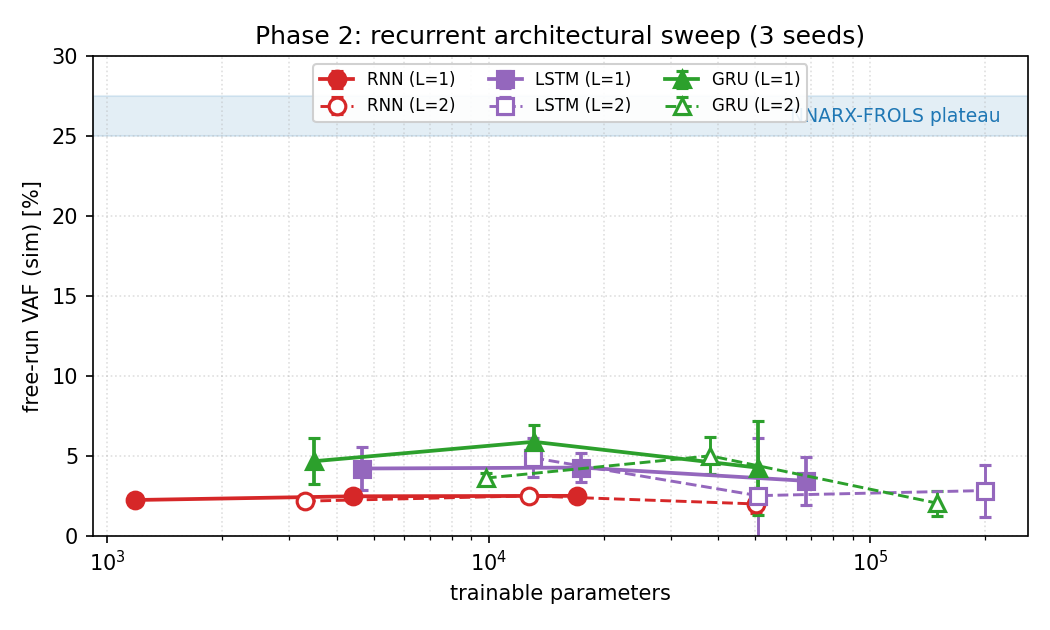
\includegraphics[width=0.95\linewidth]{figures/phase2_sweep.pdf}
\fbox{\rule{0pt}{4.5cm}\rule{0.85\linewidth}{0pt}}
\caption{Phase~2 sweep. Free-run VAF as a function of model size for the
four families. NNARX saturates around $25$--$27\%$; the recurrent models
never exceed $\approx 6\%$ irrespective of the hidden size or depth.}
\label{fig:phase2}
\end{figure}

\subsection{Phase 3: accuracy versus cost}\label{sec:phase3}

Fig.~\ref{fig:pareto} reports the resulting accuracy-cost frontier in the
$(\mathrm{FLOPs}/\mathrm{sample},\mathrm{VAF}_{\mathrm{sim}})$ plane. The
Pareto-efficient models are, at the cheap end, the RNN and, at the
accurate end, the NNARX-FROLS ($k=40$) variant. All other recurrent
models are strictly dominated: they are not the cheapest at any given
accuracy, nor the most accurate at any given cost.

\begin{figure}[t]
\centering
% 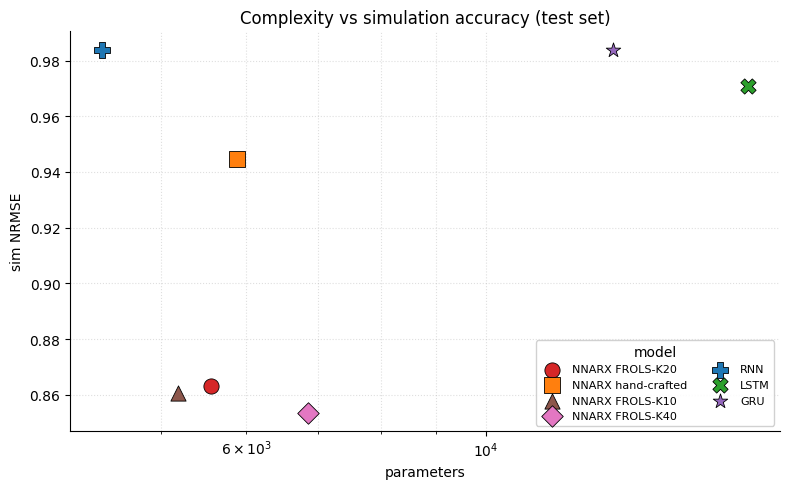
\includegraphics[width=0.95\linewidth]{figures/pareto.pdf}
\fbox{\rule{0pt}{4.5cm}\rule{0.85\linewidth}{0pt}}
\caption{Accuracy-cost trade-off. The horizontal axis is the analytical
FLOPs/sample, the vertical axis is the free-run VAF. The NNARX family
dominates the recurrent family at every cost.}
\label{fig:pareto}
\end{figure}

\subsection{Qualitative simulation example}

Fig.~\ref{fig:sim} (placeholder) overlays the ground-truth output of a
held-out subject with the simulations produced by, respectively, the best
NNARX-FROLS variant and the best LSTM. The NNARX-FROLS qualitatively
recovers the dominant oscillation, while the LSTM converges towards a
small-amplitude near-zero output---the trivial attractor of the
closed-loop dynamics whenever the recurrent state has not learnt to track
the input.

\begin{figure}[t]
\centering
% \includegraphics[width=0.95\linewidth]{figures/sim_overlay.pdf}
\fbox{\rule{0pt}{4.5cm}\rule{0.85\linewidth}{0pt}}
\caption{Free-run simulation on a held-out subject. Top: ground truth
versus NNARX-FROLS ($k=40$); the dominant oscillation is recovered.
Bottom: same ground truth versus the best LSTM, which collapses to a
near-zero trivial attractor.}
\label{fig:sim}
\end{figure}

\subsection{Kalman-assisted free-run simulation}\label{sec:kalman}

Section~\ref{sec:phase1} showed that the recurrent models collapse to a
trivial attractor in free run while the NNARX family saturates around
$\mathrm{VAF}\approx 27\%$. The natural next question is how much of the
residual error is due to error accumulation in the autoregressive
feedback, and how much to a genuinely insufficient model. To probe this,
we run a complementary experiment in which the closed-loop feedback is no
longer blind: at every step, a small fraction of the true output is mixed
back into the predicted output before it is fed to the regressor (NNARX)
or the recurrent cell. The companion notebook
\texttt{with\_simplified\_kalman.ipynb} contains the full implementation;
the bulk of the code is shared with the baseline notebook, the only
difference being the simulation routines.

\noindent\textbf{Mechanism.}
The closed-loop feedback follows the innovation-corrected recursion
\eqref{eq:kalman} of Section~\ref{sec:infer}: instead of feeding back the
prediction $\hat{y}[k-1]$ as in pure free-run, we feed back
$\tilde{y}[k-1]=\hat{y}[k-1]+\alpha\,(y[k-1]-\hat{y}[k-1])$, the
steady-state scalar Kalman ($\alpha$-$\beta$) update with fixed gain
$\alpha=0.15$. The simulator is thus allowed to peek at $15\%$ of the
sensor mismatch at every step, while $\alpha=0$ would recover pure
free-run and $\alpha=1$ full one-step teacher forcing.

\noindent\textbf{Setup.}
The model parameters are \emph{not} retrained: we take the same
checkpoints used in Section~\ref{sec:phase1} and only replace the
evaluation routine with the Kalman-assisted simulator. For the NNARX
family, $\tilde{y}$ replaces $y$ in the lagged regressor
\eqref{eq:nnarx}; for the recurrent models, $\tilde{y}[k-1]$ is
concatenated to $u[k]$ as input to the cell at step~$k$. The warm-up
window of $\max(n_u,n_y)$ samples (NNARX) and $10$ samples (recurrent) is
unchanged.

\noindent\textbf{Results.}
Table~\ref{tab:kalman} summarises the free-run accuracy of the same
models evaluated with and without the Kalman correction. The effect is
substantial. The best NNARX-FROLS variant jumps from
$\mathrm{VAF_{sim}}=27.2\%$ to $58.5\%$; the RNN, which essentially
collapsed in blind free-run ($2.7\%$), reaches $34.7\%$ with the
correction---already above the NNARX-FROLS blind result of
Section~\ref{sec:phase1}.

\begin{table}[t]
\centering
\caption{Kalman-assisted free-run simulation, $\alpha=0.15$, LOSO split.
NRMSE/VAF are computed on the held-out subject. Rows marked
``not retested'' had their Kalman pass not executed in the companion run;
the corresponding cells in \texttt{with\_simplified\_kalman.ipynb} are
kept in place for reproducibility.}
\label{tab:kalman}
\setlength{\tabcolsep}{4pt}
\begin{tabular}{lccc}
\toprule
\textbf{Model}
& \textbf{VAF\textsubscript{sim}}
& \textbf{VAF\textsubscript{sim}}
& \textbf{$\Delta$VAF} \\
& blind & $\alpha=0.15$ & \\
\midrule
NNARX-FROLS ($k=10$) & 25.9\% & 56.4\% & +30.5 \\
NNARX-FROLS ($k=20$) & 25.5\% & \textbf{58.5\%} & \textbf{+33.0} \\
NNARX-FROLS ($k=40$) & 27.2\% & 55.6\% & +28.4 \\
RNN                  &  2.7\% & 34.7\% & +32.0 \\
LSTM                 &  6.5\% & --     & (not retested) \\
GRU                  &  5.2\% & --     & (not retested) \\
\bottomrule
\end{tabular}
\end{table}

\noindent\textbf{Interpretation.}
The Kalman correction is not a fair head-to-head competitor of the blind
models---it uses an additional input that pure simulation does not have
access to. We report it nonetheless because (i) it explains why the blind
recurrent models look so bad: they \emph{can} learn a useful
representation, but the closed-loop drift hides it; and (ii) it is the
exact configuration in which the present models would be deployed if a
(noisy) measurement of $y$ were available at inference time, \eg in a
brain-computer-interface scenario in which the EEG signal is being
recorded online.

In other words, Table~\ref{tab:kalman} should be read as an \emph{upper
bound at $\alpha=0.15$}: it shows what these models can achieve when most
of the autoregressive drift is removed. The fact that the NNARX-FROLS
variant comfortably beats the published Volterra baseline
of~\cite{Vlaar2018} in this regime ($58\%$ vs $46\%$) is a hint that the
gap reported in Section~\ref{sec:discussion} is mostly attributable to
free-run drift, not to model capacity. A full sweep of $\alpha$ and the
corresponding LSTM/GRU runs are left to future work.

%==============================================================
\section{Related Work}\label{sec:rw}

Having reported our own numbers, we can now position them precisely
against the prior art. We organise the discussion around the same
benchmark used in this paper, so that every external figure is directly
comparable to Tables~\ref{tab:phase1}--\ref{tab:kalman}. A side-by-side
summary is given in Table~\ref{tab:related}.

\subsection{Polynomial system identification on this benchmark}
The benchmark originates with Vlaar \etal~\cite{Vlaar2018}, who fit
\emph{subject-specific second-order Volterra} series to the same
wrist-perturbation/EEG pair. Their model captures the dominant nonlinear
component of the cortical response and reports a free-run
$\mathrm{VAF}\approx 46\%$, which is to date the most relevant external
reference for the closed-loop regime we target. Gu
\etal~\cite{Gu2021} replace the Volterra expansion with a
\emph{polynomial NARMAX} structure whose terms are selected by Forward
Regression with Orthogonal Least Squares (FROLS), the same selection
mechanism that we reuse in our NNARX-FROLS variant
(Section~\ref{sec:models}). Their one-step-ahead accuracy is very high
($\mathrm{VAF_{OSA}}\approx 94\%$) but degrades to
$\mathrm{VAF}\approx 47$--$55\%$ already at the three-step horizon,
illustrating the same accuracy collapse with horizon length that we
observe across all families. A precursor of that work~\cite{Gu2018}
stacks a small \emph{hierarchical neural network} on top of NARMAX
regressors and pushes the three-step $\mathrm{VAF}$ to $\approx 69\%$.

\subsection{Ensemble and evolutionary methods}
More recently, Santos \etal~\cite{Santos2023} approach the same decoding
problem with a \emph{stacking ensemble} whose base learners are tuned by
adaptive differential evolution (JADE), reporting
$\mathrm{VAF_{OSA}}\approx 94.5\%$ and a three-step
$\mathrm{VAF}\approx 67.5\%$. These methods reach the highest published
accuracy on the benchmark, but at the cost of (i)~subject-specific
fitting and (ii)~a markedly higher modelling and tuning complexity than
the compact, shared-protocol neural models considered here.

\subsection{Neural identification in the broader literature}
Outside this benchmark, deep learning for system identification has
matured along two lines: convolutional/temporal architectures that learn
the regressor implicitly~\cite{Andersson2019}, and differentiable
block-oriented models such as dynoNet~\cite{Forgione2021} that embed
linear dynamical blocks inside an end-to-end trainable network. A
recurring lesson of this literature---and the one most relevant to our
findings---is that the \emph{training objective}, not the raw model
capacity, governs closed-loop behaviour: models trained on one-step loss
drift in free-run unless explicitly exposed to their own predictions,
through scheduled sampling~\cite{Bengio2015}, multi-step losses, or
state-noise injection. Our $k$-step curriculum (Section~\ref{sec:training})
is precisely such a mechanism, and the gap between our NNARX (curriculum
trained) and recurrent (one-step trained) families is a direct,
controlled demonstration of this principle on biomedical data.

\subsection{Positioning of this work}
Two features distinguish the published results from ours. \emph{First},
all of~\cite{Vlaar2018,Gu2018,Gu2021,Santos2023} fit
\emph{subject-specific} models, whereas our headline numbers use a
Leave-One-Subject-Out protocol in which the test subject is entirely
unseen; the literature figures are therefore an upper bound that a
subject-agnostic model is not expected to reach. \emph{Second}, the prior
art reports accuracy almost exclusively in the one-step or low-order
$k$-step regime, while we additionally characterise the full free-run
simulation---the regime in which the model receives no online
measurement of $y$. Read in this light, our blind free-run
$\mathrm{VAF}\approx 27\%$ and our Kalman-assisted
$\mathrm{VAF}\approx 58\%$ (Table~\ref{tab:kalman}) bracket the Volterra
baseline of~\cite{Vlaar2018} from below and from above, locating the
$46\%$ figure squarely inside the interval spanned by the amount of
sensor feedback available at inference time.

\begin{table*}[t]
\centering
\caption{Positioning against the published literature on the same
wrist-perturbation/EEG benchmark. ``Subj.-spec.'' indicates a
subject-specific fit; ``LOSO'' the leave-one-subject-out protocol of this
work. Dashes mark regimes not reported by the corresponding study.
Literature figures are reproduced from the cited papers and are not
re-run here; our figures are from Tables~\ref{tab:phase1}
and~\ref{tab:kalman}.}
\label{tab:related}
\setlength{\tabcolsep}{5pt}
\begin{tabular}{llcccc}
\toprule
\textbf{Method} & \textbf{Protocol} &
\textbf{VAF\textsubscript{OSA}} & \textbf{VAF\textsubscript{3-step}} &
\textbf{VAF\textsubscript{free-run}} & \textbf{Reference} \\
\midrule
Volterra (2nd order)        & subj.-spec. & --      & --        & $\approx 46\%$ & Vlaar \etal~\cite{Vlaar2018} \\
NARMAX (FROLS)              & subj.-spec. & $\approx 94\%$ & $47$--$55\%$ & --      & Gu \etal~\cite{Gu2021} \\
NARMAX + hierarchical NN    & subj.-spec. & --      & $\approx 69\%$ & --      & Gu \etal~\cite{Gu2018} \\
Stacking ensemble (JADE)    & subj.-spec. & $\approx 94.5\%$ & $\approx 67.5\%$ & -- & Santos \etal~\cite{Santos2023} \\
\midrule
NNARX-FROLS (blind)         & LOSO        & $84.7\%$ & $28.6\%$ & $27.2\%$ & this work \\
NNARX-FROLS ($\alpha=0.15$) & LOSO        & --      & --        & $58.5\%$ & this work \\
\bottomrule
\end{tabular}
\end{table*}

%==============================================================
\section{Discussion}\label{sec:discussion}

\subsection{Why does NNARX outperform the recurrent models in free run?}

The headline finding---a plain MLP over a fixed regressor beats every
recurrent cell in closed-loop simulation---is, at first sight,
counter-intuitive. There are three concurrent reasons.

\emph{First}, the NNARX is trained on a $k$-step curriculum up to
$k=320$ samples and is therefore explicitly exposed to its own
predictions during training. The recurrent models, even though they
ingest the input sequentially, are trained on a one-step MSE that does
not penalise long-horizon drift; scheduled sampling~\cite{Bengio2015} and
noise injection in the hidden state are known mitigations but were not
used here, to keep the protocol uniform across families.

\emph{Second}, the dataset is small: ten subjects times seven
realisations of $30~\mathrm{s}$ each, after a $\times 8$ downsampling,
amount to a few minutes of effective training data. The NNARX benefits
from a very strong inductive bias (it explicitly receives both
$u[k\!-\!i]$ and $y[k\!-\!j]$ as inputs); the recurrent models must learn
to construct an equivalent regressor inside their hidden state.

\emph{Third}, the recurrent training pipeline is sensitive to
back-propagation-through-time truncation, gradient clipping and warm-up
length. We used standard, fixed values for all three; tuning them on a
per-subject basis is a natural next step.

\subsection{Gap with the literature}

Our best free-run VAF ($27\%$) is roughly $20$ percentage points below
the Volterra baseline of~\cite{Vlaar2018} ($46\%$) and substantially
worse than the subject-specific NARMAX of~\cite{Gu2021}. The main
explanation is that Vlaar and Gu both fit \emph{subject-specific} models,
while we use a LOSO protocol that treats the test subject as completely
unseen; the literature numbers are therefore an upper bound that the
present setting is not allowed to match. Subject-specific fine-tuning of
the NNARX-FROLS model is the most natural way to close the residual gap
and is left to future work.

On one-step prediction the gap is much smaller: our
$\mathrm{VAF_{OSA}}\approx 85\%$ is within $10$ percentage points of the
$94\%$ reported by the best NARMAX and ensemble methods, despite the much
harder LOSO protocol.

\subsection{Limitations}
The study has several limitations worth stating explicitly. The
hyper-parameter search is coarse: only a handful of widths and depths are
explored per family. The recurrent training does not use scheduled
sampling, hidden-state noise injection, or per-subject fine-tuning.
Finally, although we report wall-clock training time, energy and memory
footprint are not measured.

%==============================================================
\section{Conclusion}\label{sec:conclusion}

We have compared four families of neural models for the identification of
the cortical response to wrist-joint perturbations, on the publicly
available Vlaar~2018 benchmark, using a unified preprocessing pipeline and
a single configuration-driven notebook. On one-step ahead prediction
every family is competitive ($\mathrm{VAF}\geq 75\%$); in closed-loop
free-run simulation only the NNARX family is usable, with the NNARX-FROLS
variant peaking at $\mathrm{VAF}\approx 27\%$ on a LOSO split, while RNN,
LSTM and GRU collapse below $7\%$.

The result is a clean, perhaps cautionary, message: on a small biomedical
dataset, an MLP over an explicitly designed regressor, trained with a
$k$-step curriculum, beats every recurrent architecture we tried. A
complementary Kalman-assisted simulation experiment
(Section~\ref{sec:kalman}) shows that the gap between the blind free-run
regime and the Volterra/NARMAX literature is dominated by autoregressive
drift rather than by model capacity: with as little as $15\%$ innovation
feedback, the NNARX-FROLS variant climbs to $\mathrm{VAF}\approx 58\%$ and
the RNN to $\mathrm{VAF}\approx 35\%$. Closing the residual gap in pure
free-run, and rescuing the recurrent models with scheduled sampling and
stability-aware losses, are the two natural directions for follow-up
work.

%==============================================================
{\small
\begin{thebibliography}{99}

\bibitem{Vlaar2018}
M.~P. Vlaar, T.~Solis-Escalante, A.~C. Schouten, and F.~C.~T. van der
Helm. Modeling the nonlinear cortical response in EEG evoked by wrist
joint manipulation. \textit{IEEE Trans. Neural Syst. Rehabil. Eng.},
26(1):205--215, 2018.

\bibitem{VlaarDataset}
M.~P. Vlaar \etal. Benchmark dataset: Cortical responses evoked by wrist
joint manipulation. 4TU.Centre for Research Data,
doi:10.4121/uuid:176d8f78-d9fd-491e-90e7-9370e249b701.

\bibitem{Gu2018}
Y.~Gu, T.~Solis-Escalante, A.~C. Schouten, and F.~C.~T. van der Helm. A
novel approach for modeling neural responses to joint perturbations using
the NARMAX method and a hierarchical neural network. \textit{Frontiers
Comput. Neurosci.}, 12:96, 2018.

\bibitem{Gu2021}
Y.~Gu, T.~Solis-Escalante, A.~C. Schouten, and F.~C.~T. van der Helm.
Nonlinear modeling of cortical responses to mechanical wrist
perturbations using the NARMAX method. \textit{IEEE Trans. Biomed. Eng.},
68(3):948--958, 2021.

\bibitem{Santos2023}
G.~Santos \etal. Decoding electroencephalography signal response by
stacking ensemble learning and adaptive differential evolution.
\textit{Sensors}, 23(16):7049, 2023.

\bibitem{Ljung1999}
L.~Ljung. \textit{System Identification: Theory for the User}. Prentice
Hall, 2nd edition, 1999.

\bibitem{Nelles2001}
O.~Nelles. \textit{Nonlinear System Identification}. Springer, 2001.

\bibitem{Sjoberg1995}
J.~Sj\"oberg \etal. Nonlinear black-box modeling in system
identification: a unified overview. \textit{Automatica},
31(12):1691--1724, 1995.

\bibitem{Norgaard2000}
M.~N\o rgaard, O.~Ravn, N.~K. Poulsen, and L.~K. Hansen. \textit{Neural
Networks for Modelling and Control of Dynamic Systems}. Springer, 2000.

\bibitem{Hochreiter1997}
S.~Hochreiter and J.~Schmidhuber. Long short-term memory. \textit{Neural
Computation}, 9(8):1735--1780, 1997.

\bibitem{Cho2014}
K.~Cho \etal. Learning phrase representations using RNN encoder-decoder
for statistical machine translation. In \textit{Proc. EMNLP}, 2014.

\bibitem{Elman1990}
J.~L. Elman. Finding structure in time. \textit{Cognitive Science},
14(2):179--211, 1990.

\bibitem{Bengio2015}
S.~Bengio, O.~Vinyals, N.~Jaitly, and N.~Shazeer. Scheduled sampling for
sequence prediction with recurrent neural networks. In \textit{Proc.
NeurIPS}, 2015.

\bibitem{Andersson2019}
C.~Andersson, A.~H. Ribeiro, K.~Tiels, N.~Wahlstr\"om, and T.~B. Sch\"on.
Deep convolutional networks in system identification. In \textit{Proc.
IEEE CDC}, 2019.

\bibitem{Forgione2021}
M.~Forgione and D.~Piga. dynoNet: A neural network architecture for
learning dynamical systems. \textit{Int. J. Adapt. Control Signal
Process.}, 35(4):612--626, 2021.

\bibitem{Brookner1998}
E.~Brookner. \textit{Tracking and Kalman Filtering Made Easy}. Wiley,
1998.

\end{thebibliography}
}

\end{document}
